
\chapter{Introduction}

\section{Introduction}
\subsection{Motivation}
\label{sec:motivation}
Mesenchymal stem cells might hold the promise for a great leap forward in future regenerative medicine therapies. \\
MSC can give rise to various cells found in fat- (adipocytes), cartilage- (chondrocytes), bone- (osteoblasts) and tendon-tissue (tenocytes) \cite{Barlow2008, Hass2011} and as such are important for development.
Further, they are also critical to life-long regeneration of tissue, as they persist during adult life, in different "niches", like the bone-marrow or in adipose tissue. Furthermore, they can be isolated and cultured, albeit rare in frequency. Because of this versatility, their capacity for self-renewal and their robustness, research is being done to exploit this potential for medical applications. Baek and colleagues recently described a way of ex vivo manipulating the MSCs homing behaviour before injecting them back in the donor, which stimulates migration towards injured tissue and could in the future improve recovery from myocardial infarction. \cite{Baek2011}  Additional proposals for novel applications include the fields of spinal injuries\cite{Goldschlager2010}, Multiple Sclerosis \cite{Planchon2018}, Alzheimer's Disease \cite{Han2018, Hao2012} and Diabetes \cite{Evangelista2018}.  While the promises that MSCs hold might be worthwhile, translation has been challenging. Despite the prospect of a medical revolution, currently there is no FDA approved MSC therapy available, as past proposals have been shown to either ineffective or dangerous. For example, Amariglio et al report of a dramatic account of a boy developing multiple ectopic brain tumours as a result of a faulty stem cell therapy. \cite{Amariglio2009}. Such downsides show that we need to increase our basic understanding of MSCs so that we can avoid the hazards and harness the benefits in the future.\par

The historic paradigm in cell biology that a system is described only through its biochemical status has come into question during the last years. We now know that mechanical forces, which cells experience \textit{in vivo}, influence their behaviour \cite{Hao2015}. Mechanosensing, the ability to sense forces, is a contributing factor in many cellular contexts from migration to differentiation and self-renewal. In a landmark study, Engler and colleagues\cite{Engler2006} showed that MSCs can decide on their cell fate only due to physical substrate stiffness. This study is one of many more following accounts showing that there is new, decisive knowledge in studying biophysical interaction between cells and their physical surroundings.\par

However, it is not fully understood what pathways are involved in mechanosensation of MSCs and how they regulate stem cell behaviour. More recently, the membrane-bound mechanosensitive ion-channel \Piezo{} has been described \cite{Coste2010}. The discovery marked a turning point in mechanobiology as it described the first and long sought-after eukaryotic mechanosensitive ion channel \cite{Sharif-Naeini2015}. Since then, many studies have corroborated the idea of \Piezo{} belonging to a family of receptors who have already been predicted to exist since 1950 \cite{Katz1949}. While we now know that \Piezo{} is involved in neural stem cell differentiation \cite{Pathak2014} and vascular development \cite{Ranade2014}, it is not fully understood how \Piezo{} influences MSC behaviour. \par
In this work, we investigate the importance of \Piezo{} in MSC mechanosensing and shed light on its influence regarding ECM turnover and differentiation.


DRAFT: 


The existence of MechanICs was already postulated in 1950 in a study measuring a change of electric potential in response to stretching of muscle \cite{Katz1949}. Over the years, the existence of MechanICs became increasingly clear, as studies showed them to contribute to a variety of physiological functions, like regulating the myogenic tone of resistance arteries in muscle \cite{Murthy2017} or stimulation of vasodilatation in the vascular system \cite{Zeng2018}. Especially, in pain research, were neurons implicated in pain sensation seem to rely on MechanICs, the necessity for discovery was urgent. Notwithstanding the relevance, the discovery of the first gene encoding a MechanIC would take another 44 years, until Sukharev and colleagues describe two distinct genes mscL and mscS, whose product mediate stretch sensing in the membrane of E. Coli bacteria. While the efforts and papers, that were inspired by this discovery, gave great insight into structure and biophysical mechanism of those channels, eukaryotic homologues were still missing. Until recently, the only eukaryotic candidate was TREK-1, a potassium-selective ion channel, whose mechanosensitive property is still controversial. 

Tendon is collagenous and highly tensile tissue that connects muscle to bone, acting as a force transmission and effectively enabling us to move. 

Add Comment about tendon metabolism. 

The well-being of our tendon is crucial, as patients with tendon-related diseases suffer a lot and they are increasing in number with a projected amount of XX Patients in 20XX. The most prevalent tendon related disease next to rupture is called tendinopathy and describes an inflammatory disease of the tendon, with most common symptoms reported being movement associated pain, swelling and substantial decrease in quality of life. On a clinical level erroneous blood vessel formation inside the normally non-vascularized tendon core (vascular in-growth) is the hallmark of this disease. Currently, the pathophysiology is poorly understood. This lack of understanding regarding tendinopathy etiology leads to the treatment being largely symptomatic. 

Some cases progress and make surgical intervention necessary. In those cases, the surgeon can cut out the diseased part, hence the need for tendon replacement surgery.  One approach is to transfer tendon from a non-diseased site. *Explain Problems that we are left with and how mesenchymal stem cells can help us* They hold great promises, but systematic success is still lacking. This is largely due to undefined behaviour. *Explain reasons for why they do not work now* 

More and more, it becomes clear that we need to understand the dynamics better that underlie MSCs before we can start utilizing their full potential.\par 

Mechanobiology is this domain of biology at the interface between cells and their physical environment. 
Even though the first hypothesis that involve cells being able to sense physical stimuli dates back to the late 19th century, the pathways implicated in mechanobiology are heavily researched and mechanobiology is rather recently gaining a lot of scientific momentum. Eyckman and colleagues suggest a lack in technology as main reason for this delay from conceptualisation to investigation \cite{Eyckmans2011}. 
The identification of mechanically gated channel (MechanIC) named \Piezo{} was very important to push the frontier of the field. \par
\Piezo{} is a calcium-permeable non-selective ion-channel located at the membrane. Its discovery in 2009 marks a groundbreaking advancement for mechanobiology and cell biology in general as it is the first description of a mechanosensitive ion channel found in eukaryotic cells.\cite{Coste2010} 
Finally, in their breakthrough paper from 2010, Coste and colleagues report the discovery of two genes Fam38A and Fam38B, which encode mechanosensitive protein Piezo1 and Piezo2, respectively. Even though they carefully avoided calling Piezo1 an ion channel in their first paper, a follow-up study in the same lab confirmed piezo proteins as subunits for the homo-trimeric MechanIC Piezo1. Finally, scientists characterized the first eukaryotic mechanosensitive ion channel. 




\section{Theory}

\subsection{\Piezo{}}

\begin{figure}
	\centering
	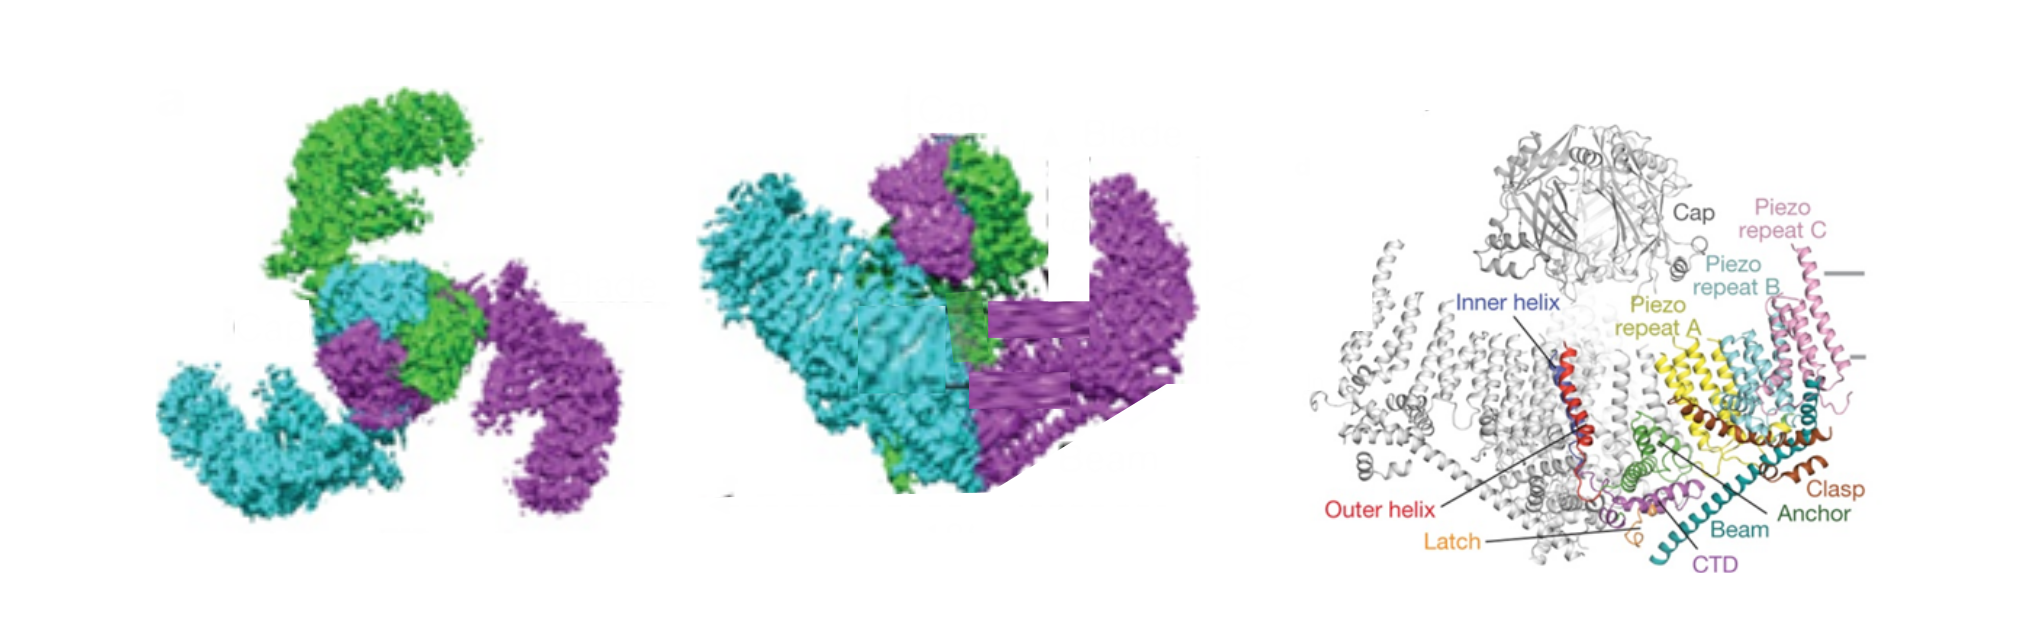
\includegraphics[width=0.6\linewidth]{PiezoMolecule.png}
	\caption{Molecular structure of \Piezo{} as assessed by cryo-EM analysis. Top (left) and side (middle) view of \Piezo{} and cartoon representation of \Piezo{} with important domains highlighted (right). Adapted from \cite{Saotome2018, Zhao2018}.}
	\label{pic:Piezo}
\end{figure}

\Piezo{} and \textsc{Piezo2} are the only known members of the \textsc{Piezo}-family. 
The protein family is genetically and structurally unique, as the similarity to other proteins are minimal \cite{Coste2010}. 
\Piezo{} can be found in various tissues and cell types throughout the body and constitutes the mechanosensitive homo-trimeric cation channel \Piezo{} \cite{Zhao2018}. \Piezo{} is evolutionary conserved as homologues span the whole division of multicellular animals (Metazoa). Intriguingly, the uniqueness also translates to the architecture of the channel as shown in work done by Saotome and colleagues giving great insight into \Piezo{}-structure using cryo-EM analysis \cite{Saotome2018}. The large channel comprises a central pore in the middle with a three-bladed propeller like structure facing the extracellular space (\myworries{see Fig.} \ref{pic:Piezo}). \Piezo{} resides on the membrane in a closed state. The activation sequence start with the cellular membrane being exposed to a mechanical force exceeding a certain threshold, which leads to \Piezo{} switching into an open state where it allows calcium and other cations to enter the intracellular space, before reverting into an inactive state, where the channel is non-responsive to stimuli. After a relaxation period, the channel switches back to a responsive, closed state. While the exact activation mechanism remains elusive, there is evidence for the mechanotransductory chain starting with force-mediated bending of blades which then transmits the tension over anchor/beam region, leading to the opening of a previously allosterically closed inner portion of the cation channel \cite{Zhao2018}. This hypothesis is corroborated by findings that blades exhibit flexibility over many different bending modes, which supports the notion of the blades being the mechanosensory unit of the channel \cite{Ge2015}. 
Research on mechanosensitive ion channels and \Piezo{} relied on physical activation techniques, like application of physical forces or the patch clamp technique. Alternatively, \Piezo{} can be activated by a small chemical \Piezo{}-agonist, called \Yoda{} (a nod towards movie director George Lucas’ use of “the Force”). \Yoda{} has been shown to chemically activate \Piezo{} by acting as a molecular wedge, without eliciting a similar response in other channels \cite{Syeda2015, Lacroix2018}. Therefore, \Yoda{} can be used to study the influence of \Piezo{} in an isolated design \cite{Botello-Smith2019}.

\subsection{Bone Marrow-derived Mesenchymal Stem Cells}

Mesenchymal stem cells (MSCs) are characterized by four different properties: First, they hold the potential to differentiate into a defined set of cells, including osteocyte (bone), chondrocyte (cartilage), adipocyte (fat-tissue) and tenocyte (tendon) \cite{Ng2008}. Second, they hold the potential to self-renew, meaning they can give rise to identical cells. Third, they expose a set of stem cell markers like CD31, CD34 and cKit, which are associate with but not unique to MSCs. \cite{Battula2009} And fourth, they can be conveniently isolated from primary tissue based on their capacity to stick on plastic. \cite{Buhring2007}. Furthermore, there is a growing body of evidence that attributes an immunomodulatory effect of MSC on injured or inflamed sites, which could relate to better outcome in medical intervention \cite{Caplan2011, Hass2011}.
While there are differing anatomical sources where mesenchymal stem cells can be isolated from, including the umbilical cord and adipose tissue \cite{Barlow2008, Hass2011} in this work we focus on human bone-marrow derived mesenchymal stem cells and from now on will refer to them as mesenchymal stem cells (MSCs).

\begin{itemize}
	\item Also give a little introduction about MSC niche. 
\end{itemize}

\subsection{Mechanobiology of MSCs}

Although we have made substantial progress in our understanding of the chemical cues that are important to MSC behaviour, there is a gap in our knowledge how mechanical signals are involved. It becomes increasingly clear that mechanical signal are also potent regulators of MSC behaviour. 


\begin{itemize}
	\item MSCs being largely influenced by physical forces. Physiological pressure ranges are.
	\item need to include YAP. 
	\item Cytoskeleton naturally in a state of tensile forces (Tensegrity, Brown2010). These lead to pull on the surrounding ECM. 
	\item Although advancements in our understanding of biochemical cues critical to stem cell function have been made, there is a significant gap in our understanding of how mechanical signals are involved.
	\item Avian embryos that are completely paralyzed, show weird growth in muscles and bone.
	\item Compressive forces induce chondrogenic differentiation, tensile induce osteogenic diff.
	\item OSteogenic diff also possible through right ECM From Brown: These data support the idea that intracellular tensile forces resulting from cell– ECM interactions are potent enough to induce differentiation and small forces may be just as critical as larger external forces in directing stem cell fate. Ruiz and Chen
	\item (16): They later showed that human MSCs seeded as multicellular aggregates in wells and cultured in adipo-osteogenic media, differentiated into adipocytes and osteoblasts depending on their location within the matrix and the corresponding stress level	
	\item BROWN: They later showed that human MSCs seeded as multicellular aggregates in wells and cultured in adipo-osteogenic media, differentiated into adipocytes and osteoblasts depending on their location within the matrix and the corresponding stress level [16••]. Cells growing in regions of low stress, at the center of the matrix, differentiated into adipocytes, whereas cells growing in regions of high stress, at the edges of the matrix, differentiated into osteoblasts. This striking pattern mimics tissue arrangement in living bone where fat-containing marrow is surrounded by a mineralized cortical shell comprised of osteoblasts. 
	\item This is interesting because it could have potentially impact on recommendation of loading during bone healing. Sheep Paper: "The influence of induced micro- movement upon the healing of experimental tibial fractures."
	\item Different modalities how cells feel, are changes in cytoskeleton, connections to ECM and membrane-bound channels
	\item One of them being Piezo1	
	
	
\end{itemize}

This text discusses with not more than 500 words the mechanobiological properties of different MSCs niches. Also it sheds light on how those led to mechanobiological studies, that found particularly noteworthy discoveries. \par

Reviews:
\begin{itemize}
	\item Brown et al (2019): Mesenchymal stem cells: Cell therapy and regeneration potential
	\item Castillo \& Jacobs (2010): Mesenchymal Stem Cell Mechanobiology
\end{itemize}


\subsection{\Piezo{}}

\begin{figure}
	\centering
	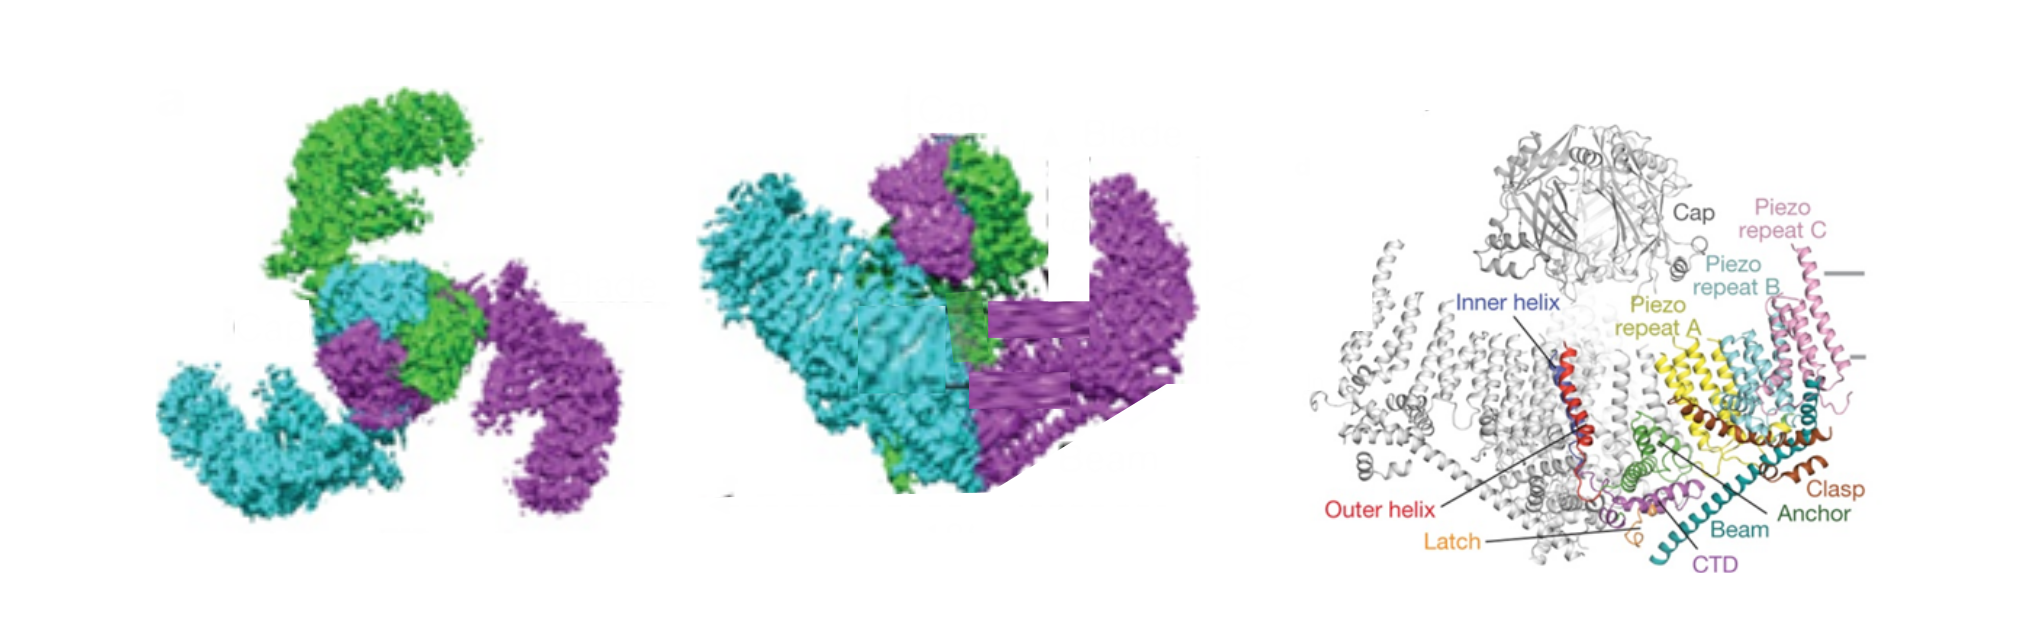
\includegraphics[width=0.6\linewidth]{PiezoMolecule.png}
	\caption{Molecular structure of \Piezo{} as assessed by cryo-EM analysis, adapted from \cite{Saotome2018, Zhao2018}.}
	\label{pic:Piezo}
\end{figure}

\Piezo{} and \textsc{Piezo2} are the only known members of the \textsc{Piezo}-family. 
The protein family is genetically and structurally unique, as the similarity to other proteins are minimal \cite{Coste2010}. 
The ubiquitously expressed protein \Piezo{} constitutes the mechanosensitive homo-trimeric cation channel \Piezo{} \cite{Zhao2018}. \Piezo{} is evolutionary conserved as homologues span the whole division of multicellular animals (Metazoa). Intriguingly, the uniqueness also translates to the architecture of the channel as shown in an very elegant paper by Saotome and colleagues giving insight into \Piezo{}-structure using cryo-EM analysis \cite{Saotome2018}. The large channel comprises a central pore in the middle with a three-bladed propeller like structure facing the extracellular space. \Piezo{} resides on the membrane in a quiescent, closed state. The activation sequence start with the cellular membrane being exposed to a mechanical force exceeding a certain threshold, which leads to \Piezo{} switching into an open state where it allows calcium and other cations to enter the intracellular space, before reverting into an inactive state, where the channel is non-responsive to stimuli. After relaxation period it switches back to a responsive, closed state. While the exact activation mechanism remains elusive, there is evidence for the mechanotransductory chain starting with force-mediated bending of blades which then transmits the tension over anchor/beam region, leading to the opening of a previously allosterically closed inner portion of the cation channel \cite{Zhao2018}. This hypothesis is corroborated by findings that blades exhibit flexibility over many different bending modes, which supports the notion of the blades being the mechanosensory unit of the channel \cite{Ge2015}. 
Research on mechanosensitive ion channels and \Piezo{} relied on physical activation techniques, like application of physical forces or the patch clamp technique. However, these methods don’t fully accommodate the sensitivity that is needed , when one intends to measure the contribution of a single channel type. \cite{Dubin2017} Alternatively, in research we have access to a chemical \Piezo{}-agonist, called \Yoda{} (a nod towards movie director George Lucas’ use of “the Force”). \Yoda{} has been shown to chemically activate \Piezo{} by acting as a molecular wedge, without eliciting a similar response in other channels \cite{Syeda2015, Lacroix2018}. Therefore, \Yoda{} can be used to study the influence of \Piezo{} in an isolated design \cite{Botello-Smith2019}.
